\chapter{La CyberSécurité et La Sécurité Informatique}
\section{La CyberSécurité}
\subsection{Définition}
\paragraph{ }
La cybersécurité, également appelée sécurité informatique ou sécurité des technologies de l'information, est l'ensemble des mesures techniques, organisationnelles et juridiques mises en place pour protéger les systèmes informatiques, les réseaux et les données contre les attaques, les pertes ou les altérations. Elle vise à garantir la confidentialité, l'intégrité et la disponibilité des informations stockées sur les systèmes informatiques, ainsi que la protection de la vie privée et des droits de propriété intellectuelle.
\paragraph{ }
La cybersécurité concerne la sécurité informatique et des réseaux des environne-
ments connectés à Internet et accessibles via le cyberespace. Elle peut être mise en
défaut, entre autres, par des cyberattaques informatiques. Du fait de l’usage extensif
d’Internet, de nouvelles menaces sont apparues générant des risques additionnels
dont les impacts, de niveaux d’importance variables, peuvent affecter les individus,
les organisations ou les États. 
\paragraph{ }
La cybersécurité est devenue un enjeu majeur dans le monde numérique d'aujourd'hui, où les attaques informatiques sont de plus en plus sophistiquées et fréquentes. Elle est essentielle pour protéger les systèmes informatiques et les données sensibles contre les menaces potentielles et assurer la continuité des activités des organisations qui les utilisent. La cybersécurité est également importante pour protéger les utilisateurs finaux, tels que les consommateurs et les employés, contre les risques de vol d'identité, de fraude en ligne et d'autres formes de cybercriminalité.
\paragraph{ }
Les points essentiels englobés par la cybersécurité comprennent :
\space \paragraph{ }


\paragraph{1. La confidentialité :}\paragraph{} la protection des données contre les accès non autorisés. Cela inclut la protection des données personnelles, des secrets commerciaux, des informations financières et autres informations sensibles.

\paragraph{2. L'intégrité :}\paragraph{} la protection des données contre les altérations non autorisées. Cela inclut la garantie que les données sont exactes et fiables.

\paragraph{3. La disponibilité :} \paragraph{}la garantie que les systèmes, les réseaux et les données sont accessibles et fonctionnent correctement, et que les interruptions de service sont minimisées.

\paragraph{4. L'authenticité:}  \paragraph{}la garantie que les utilisateurs sont bien ceux qu'ils prétendent être, et que les données sont bien celles qu'elles prétendent être.

\paragraph{5. La non-répudiation: } \paragraph{}la garantie qu'une personne ne peut pas nier avoir effectué une action ou avoir envoyé des données.

\paragraph{6. La résilience :} \paragraph{}la capacité des systèmes et des réseaux à résister aux attaques et à récupérer rapidement en cas d'incident.
\pagebreak

\paragraph{7. La conformité :} \paragraph{}le respect des lois, des réglementations et des normes en matière de sécurité informatique.

\paragraph{8. La sensibilisation :}\paragraph{} l'éducation et la formation des utilisateurs pour qu'ils comprennent les risques liés à la sécurité informatique et les meilleures pratiques à suivre pour les éviter.

Ces points essentiels sont interconnectés et doivent être pris en compte dans toute stratégie de cybersécurité efficace.
\section{La Sécurité Informatique }
\subsection{Définition}
 \section{La Securite Informatique }


\paragraph{ }  La sécurité informatique est l'ensemble des mesures techniques, organisationnelles et juridiques mises en place pour protéger les systèmes informatiques, les réseaux et les données contre les attaques, les pertes ou les altérations. Elle vise à garantir la confidentialité, l'intégrité et la disponibilité des informations stockées sur les systèmes informatiques, ainsi que la protection de la vie privée et des droits de propriété intellectuelle.  

\paragraph{ } La sécurité informatique englobe un large éventail de domaines, tels que la sécurité des réseaux, la sécurité des systèmes d'exploitation, la sécurité des applications, la sécurité des données, la sécurité physique, la gestion des identités et des accès, la conformité aux normes de sécurité, la surveillance et la détection des incidents de sécurité, ainsi que la réponse aux incidents de sécurité.

\paragraph{ }  La sécurité informatique est devenue un enjeu majeur dans le monde numérique d’aujourd’hui, où les attaques informatiques sont de plus en plus sophistiquées et fréquentes. La mise en place d'une politique de sécurité informatique efficace est donc essentielle pour protéger les systèmes informatiques et les données sensibles contre les menaces potentielles et assurer la continuité des activités des organisations qui les utilisent.
\pagebreak

\hbox{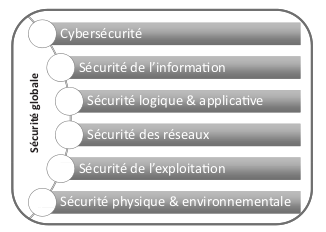
\includegraphics[width=0.5\textwidth]{image_sec.png}}
\paragraph{ }
\hbox{ La sécurité informatique englobe plusieurs domaines d'applications :}
\vspace{5mm}
\textendash \space   sécurité physique et environnementale ;
\paragraph{ }
\textendash \space   sécurité de l’exploitation ;
\paragraph{ }
\textendash \space  sécurité des réseaux ;
\paragraph{ }
\textendash \space  sécurité logique, sécurité applicative et sécurité de l’information ;
